\documentclass[brazil]{beamer}
\usepackage{pacotesLaTeX}

\title{Cadeia de Ising com campo transverso}
\author{Thales Freitas Macêdo}  

\begin{document}

\frame{\titlepage}

\begin{frame}{Modelo de Ising clássico}
    O modelo de Ising é um modelo de spins \( S_i = \pm 1 \) localizados, formando uma rede,
    sob ação de um campo magnético externo \( H \), alinhado com os spins.
    \[ E = - J \sum_{\expval{ij}} S_i S_j - \mu H \sum_i S_i \]
\end{frame}

\begin{frame}{Cadeia de Ising com campo transverso}
    O modelo de Ising com campo transverso é obtido ao impor que a direção do campo magnético
    seja transversa à direção dos spins.
    Agora, não podemos mais tratar o problema classicamente, e temos que usar a mecânica quântica.
    Vou abordar o problema unidimensional da cadeia de Ising.
    \begin{equation}
        H = - \sum_i \qty[\Gamma S_i^x + J S_i^z S_{i + 1}^z] = - \sum_i \qty[S_i^x + \lambda S_i^z S_{i + 1}^z] \label{hamiltoniano}
    \end{equation}
    onde \( S^\alpha \) é o operador de spin de Pauli na direção \( \alpha \), \( J \) é a constante de interação entre os spins,
    \( \Gamma \) é a constante do campo, e \( \lambda = J / \Gamma \), com \( \Gamma = 1 \).
\end{frame}

\begin{frame}{Cadeia de Ising com campo transverso}
    Definimos o gap de massa \( \Delta (\lambda) \) como a diferença de energia entre o estado fundamental e o primeiro estado excitado.
    Numa transição de fase quântica, \( \Delta = 0 \), e o comprimento de correlação \( \xi = 1 / \Delta \) diverge.
\end{frame}

\begin{frame}{Método \textit{Finite-Size Scaling}}
    Nesse método, diagonalizamos exatamente o Hamiltoniano para cadeias com \( N = 2, 3, 4, \dots \) spins.
    A princípio, uma cadeia com muitos spins aproximaria o limite termodinâmico \( N \to \infty \) mais adequadamente,
    mas pode ser numericamente muito custoso.
    Podemos usar a seguinte relação para estimar os parâmetros no limite termodinâmico:
    \begin{equation}
        \lambda_c (L) = \lambda_c + A L^{-1/\nu} ,
    \end{equation}
    onde \( \lambda_c \) é valor crítico de \( \lambda \) para uma transição de fase quântica, \( L \) representa os tamanhos das cadeias,
    \( A \) é uma constante e \( \nu \) é um expoente crítico relacionado ao comprimento de correlação \( \xi \).
\end{frame}

\begin{frame}{Método \textit{Finite-Size Scaling}}
    Na base de autovalores de \( S^x \), as representações matriciais de \( S^\alpha \) para o espaço de 1 spin são
    \begin{equation}
        S^x = \mqty(
        1 & 0 \\
        0 & -1
        )
    \end{equation}
    e
    \begin{equation}
        S^z = \mqty(
        0 & 1 \\
        1 & 0
        ) .
    \end{equation}
    Temos agora que obter uma representação matricial dos operadores \( S_i^\alpha \).
\end{frame}

\begin{frame}{Método \textit{Finite-Size Scaling}}
    No espaço de estados de \( N \) spins, temos que fazer o produto tensorial entre \( S_i^\alpha \) e operadores identidade para os outros spins.
    A representação do produto tensorial desses operadores é obtido pelo produto de Kronecker:
    \begin{equation}
        \vb{A} \otimes \vb{B} = \mqty(
        a_{11} \vb{B} & \dots & a_{1n} \vb{B} \\
        \vdots & \ddots & \vdots \\
        a_{m1} \vb{B} & \dots & a_{mn} \vb{B}
        )
    \end{equation}
\end{frame}

\begin{frame}{Método \textit{Finite-Size Scaling}}
    Por exemplo, se \( N = 4 \):
    \begin{equation}
        H = - \qty(S_1^x + S_2^x + S_3^x + S_4^x) - \lambda (S_1^z S_2^z + S_2^z S_3^z + S_3^z S_4^z) .
    \end{equation}
    Para estabelecer condições de contorno periódicas, basta adicionar o termo \( - \lambda S_4^z S_1^z \).
\end{frame}

\begin{frame}{Método \textit{Finite-Size Scaling}}
    Encontrei o gap de massa para os casos \( N = 2, 3, 4, 5, 6, 7, 8, 9, 10 \):
    \begin{figure}
        \centering
        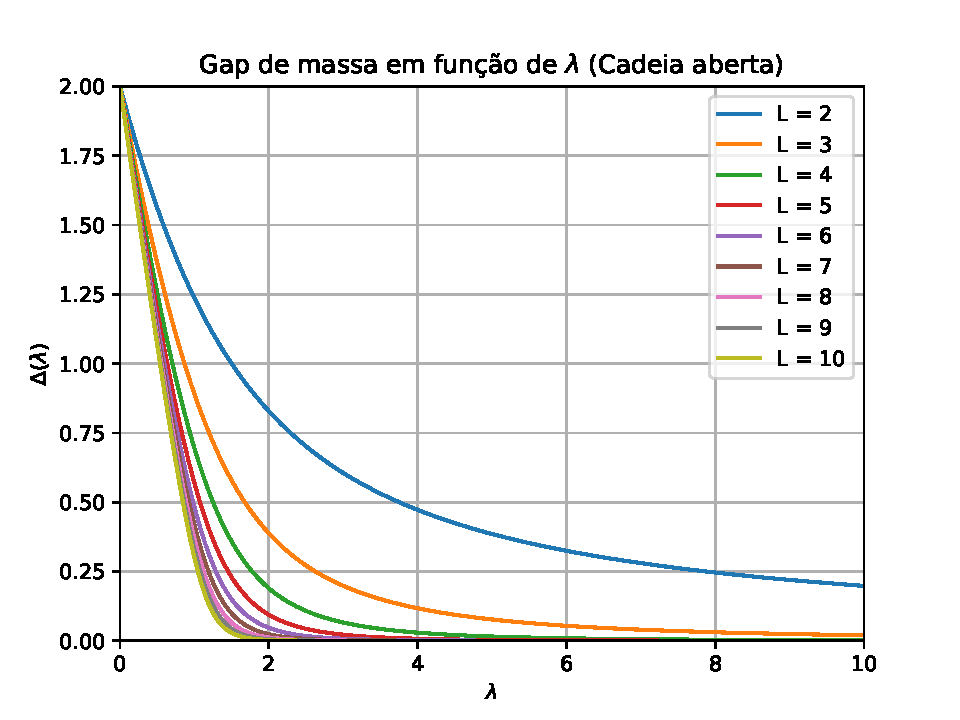
\includegraphics[width=0.7\textwidth]{gap.pdf}
    \end{figure}
\end{frame}

\begin{frame}{Método \textit{Finite-Size Scaling}}
    Encontrei o gap de massa para os casos \( N = 2, 3, 4, 5, 6, 7, 8, 9, 10 \):
    \begin{figure}
        \centering
        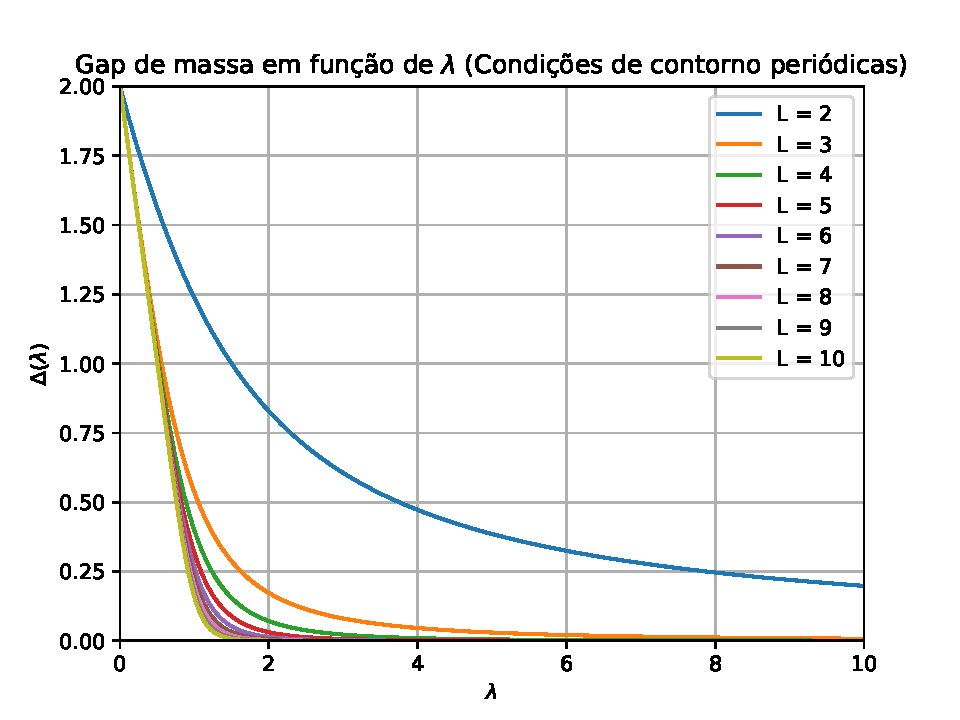
\includegraphics[width=0.7\textwidth]{gap_ccp.pdf}
    \end{figure}
\end{frame}

\begin{frame}{Método \textit{Finite-Size Scaling}}
    Os gaps de massa tendem a zero no infinito para cadeias finitas.
    Só há transição de fase quântica no limite termodinâmico.
    Temos que estimar de alguma forma \( \lambda_c \) para os casos finitos.
    Uso a razão de gap de massa:
    \begin{equation}
        R_L = \frac{L \Delta(\lambda, L)}{(L - 1) \Delta (\lambda, L - 1)} .
    \end{equation}
    O parâmetro crítico \( \lambda_c \) pode ser aproximado como
    a solução da equação \( R_L (\lambda_c) = 1 \).
\end{frame}

\begin{frame}{Método \textit{Finite-Size Scaling}}
    Calculei os \( \lambda_c \) e plotei em função de \( L \):
    \begin{figure}
        \centering
        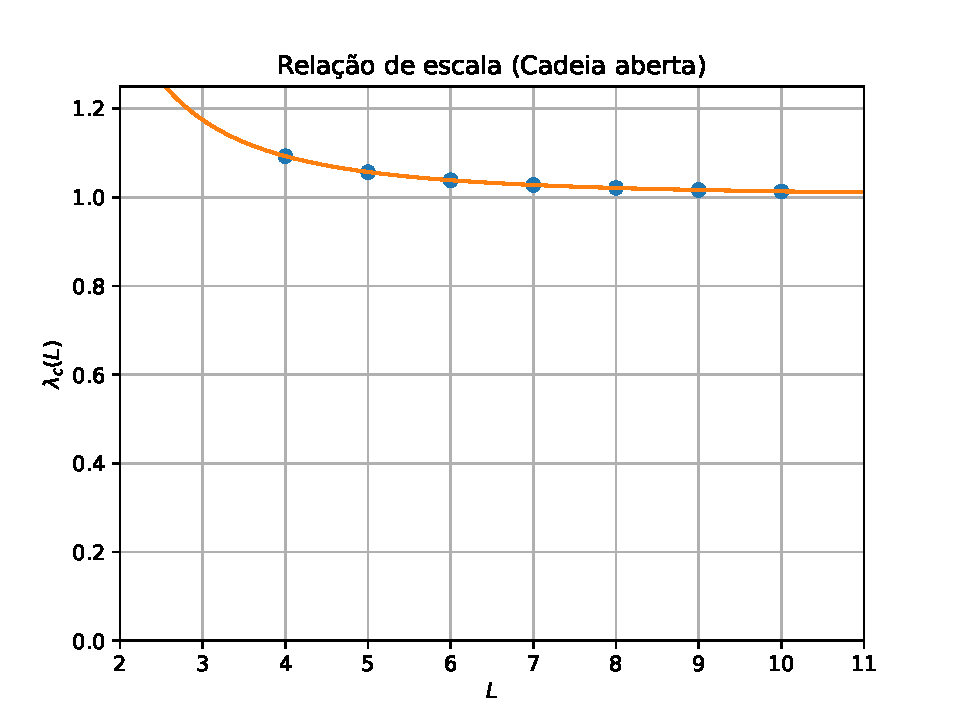
\includegraphics[width=0.7\textwidth]{rel_escala.pdf}
    \end{figure}
    O ajuste à função \( f(x) = c + A x^k \) forneceu
    \begin{align*}
        c = \num{1.0013(2)} & & A = \num{1.98(3)} & & k = \num{-2.22(1)}
    \end{align*}
\end{frame}

\begin{frame}{Método \textit{Finite-Size Scaling}}
    Calculei os \( \lambda_c \) e plotei em função de \( L \):
    \begin{figure}
        \centering
        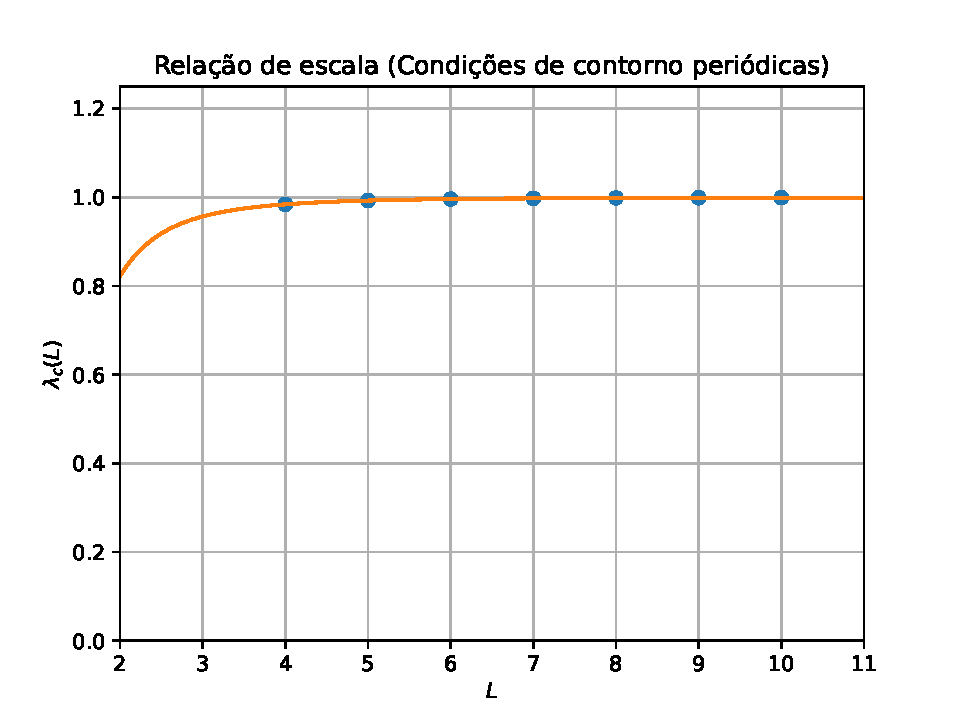
\includegraphics[width=0.7\textwidth]{rel_escala_ccp.pdf}
    \end{figure}
    O ajuste à função \( f(x) = c + A x^k \) forneceu
    \begin{align*}
        c = \num{0.99984(3)} & & A = \num{-2.01(5)} & & k = \num{-3.50(2)}
    \end{align*}
\end{frame}

\begin{frame}{Método \textit{Block Renormalisation Group}}
    A ideia por trás do método é gerar um procedimento iterativo que produza o Hamiltoniano (\ref{hamiltoniano}) na \( n \)-ésima iteração
    \begin{equation}
        H^{(n)} = - \sum_i \qty( J^{(n)} S_i^{z (n)} S_{i + 1}^{z (n)} + \Gamma^{(n)} S_i^{x (n)} ) + c^{(n)} \sum_i I_i^{(n)} ,
    \end{equation}
    com as condições iniciais \( J^{(0)} = J \), \( \Gamma^{(0)} = \Gamma \) e \( c^{(0)} = 0 \).
\end{frame}

\begin{frame}{Método \textit{Block Renormalisation Group}}
    Começamos dividindo a cadeia de \( N \) sítios em \( N / b \) blocos com \( b \) spins em cada bloco e
    reescrevemos o Hamiltoniano como a soma de uma parte intra-bloco \( H_B \) e outra inter-bloco \( H_{IB} \), com
    \begin{equation}
        H_B = \sum_{p = 1}^{N / b} H_p \qc H_{IB} = \sum_{p = 1}^{N / b - 1} H_{p, p + 1}
    \end{equation}
    com
    \begin{align}
         & H_p = - \sum_{i = 1}^{b - 1} J S_{i, p}^z S_{i + 1, p}^z + \Gamma \sum_{i = 1}^b S_{i, p}^x \\
         & H_{p, p + 1} = - J S_{n, p}^z S_{1, p + 1}^z
    \end{align}
    onde os índices \( i \) e \( p \) se referem ao \( i \)-ésimo spin no \( p \)-ésimo bloco.
\end{frame}

\begin{frame}{Método \textit{Block Renormalisation Group}}
    Diagonalizamos o Hamiltoniano \( H_p \), obtendo os estados fundamental \( \ket{0} \)
    e primeiro excitado \( \ket{1} \), de energias \( E_0 \) e \( E_1 \).
    Para efetuar o processo de renormalização, introduzimos um novo conjunto de operadores de spin \( S_p^{\alpha (1)} \)
    associado ao bloco \( p \), tal que os autoestados de \( S_p^{x (1)} \) sejam \( \ket{0} \) e \( \ket{1} \).
    Assim, podemos reescrever \( H_p \), na primeira iteração, na forma renormalizada
    \begin{equation}
        H_p^{(1)} = - \Gamma^{(1)} S_p^{x (1)} + c^{(1)} I_p^{(1)} ,
    \end{equation}
    onde
    \begin{equation}
        \Gamma^{(1)} = \frac{E_1 - E_0}{2} \qc c^{(1)} = \frac{E_1 + E_0}{2} .
    \end{equation}
\end{frame}

\begin{frame}{Método \textit{Block Renormalisation Group}}
    Para reescrever o Hamiltoniano total na forma renormalizada, incluímos a parte inter-bloco de forma perturbativa.
    % Em ordem zero, \( H^{(1)} = H_p^{(1)} \). Em primeira ordem, tomando o elemento de matriz de \( S_{i, p}^z \) entre os estados \( \ket{0} \) e \( \ket{1} \),
    % \begin{equation}
    %     H_{p, p + 1}^{(1)} = - J^{(1)} \sum_p S_p^{z(1)} S_{p + 1}^{z(1)}
    % \end{equation}
    % onde
    % \begin{equation}
    %     J^{(1)} 
    % \end{equation}
    Assim obtemos as relações de recursão para a (\( n + 1 \))-ésima iteração,
    \begin{align}
         & \Gamma (n + 1) = \frac{E_1^{(n)} - E_0^{(n)}}{2}                 \\
         & J (n + 1) = \qty( \eta_1^{(n)} )^2 J^{(n)}                       \\
         & c(n + 1) = b c^{(n)} + \frac{E_1^{(n + 1)} + E_0^{(n + 1)}}{2} .
    \end{align}
\end{frame}

% \begin{frame}{Método \textit{Block Renormalisation Group}}
%     Para realizar a descrição numérica desse problema uso o método do grupo de renormalização.
%     Para exemplificar o método, apresento o grupo de renormalização de bloco de spin de Kadanoff.
%     \begin{columns}
%         \begin{column}{0.5\textwidth}
%             \begin{figure}
%                 \includegraphics[width=\textwidth]{Rgkadanoff.png}
%             \end{figure}
%         \end{column}
%         \begin{column}{0.5\textwidth}
%             Começamos ao dividir o sólido em blocos \( 2 \times 2 \).
%             Usamos variáveis de bloco, que descrevem o comportamento médio do bloco.
%             Usamos a aproximação de que as variáveis de bloco obedecem a uma hamiltoniana do mesmo formato do sistema original.
%         \end{column}
%     \end{columns}
% \end{frame}

% \begin{frame}{Método \textit{Block Renormalisation Group}}
%     \begin{columns}
%         \begin{column}{0.5\textwidth}
%             \begin{figure}
%                 \includegraphics[width=\textwidth]{Rgkadanoff.png}
%             \end{figure}
%         \end{column}
%         \begin{column}{0.5\textwidth}
%             Com menos átomos envolvidos, o problema se torna mais fácil de resolver.
%             Podemos iterar sobre diferentes tamanhos de blocos, em busca de pontos fixos.
%         \end{column}
%     \end{columns}
% \end{frame}

\begin{frame}
    \frametitle{Referências}
    \nocite{*}
    \bibliographystyle{plain}
    % \bibliographystyle{amsalpha}
    \bibliography{refs}
\end{frame}

% \bibliography{refs} % Entries are in the refs.bib file

\end{document}
